% =====================================================================
% LMA Individual Project -- consolidated final report (Phases 1-3).
%
% Compile with XeLaTeX, twice:   bash report/final/build.sh
% Needs a Devanagari-capable font (Nirmala UI on Windows).
% Figures: report/final/make_final_figures.py regenerates every PDF in
% report/final/figures/ from the result artifacts.
%
% Hard limit: 10 pages.
% =====================================================================
\documentclass[10pt]{article}

\usepackage[margin=0.72in]{geometry}
\usepackage{amsmath}
\usepackage{amssymb}
\usepackage{fontspec}
\usepackage{graphicx}
\usepackage{booktabs}
\usepackage{array}
\usepackage{xcolor}
\usepackage{caption}
\usepackage{subcaption}
\usepackage{float}
\usepackage{enumitem}
\usepackage{tikz}
\usetikzlibrary{positioning, arrows.meta, fit, backgrounds}

\captionsetup{font=small, labelfont=bf, skip=2pt}
\setlength{\textfloatsep}{6pt}
\setlength{\intextsep}{6pt}
\setlength{\abovecaptionskip}{3pt}
\setlength{\belowcaptionskip}{0pt}
\PassOptionsToPackage{hyphens}{url}
\usepackage[colorlinks=true, linkcolor=blue!50!black, urlcolor=blue!50!black,
            citecolor=blue!50!black]{hyperref}
\emergencystretch=3em
\sloppy

% Devanagari. Nirmala UI ships with Windows; Noto Sans Devanagari elsewhere.
\newfontfamily\devanagarifont{Nirmala UI}
\newcommand{\dn}[1]{{\devanagarifont #1}}

\graphicspath{{figures/}{../phase1/figures/}{../phase2/figures/}{../phase3/figures/}}

\usepackage{titlesec}
\titlespacing*{\section}{0pt}{4pt}{1.5pt}
\titlespacing*{\subsection}{0pt}{3pt}{0.5pt}
\titleformat*{\subsection}{\normalsize\bfseries}
\setlength{\parskip}{1.1pt}
\setlength{\tabcolsep}{4.5pt}
\renewcommand{\arraystretch}{0.93}
\setlist[itemize]{topsep=1pt, itemsep=0.5pt, parsep=0pt, leftmargin=12pt}

% Shared TikZ vocabulary for the three pipeline diagrams.
\tikzset{
  stage/.style  = {draw=black!55, rounded corners=1.6pt, fill=black!4,
                   inner sep=2.6pt, align=center, font=\scriptsize, minimum height=12pt},
  hstage/.style = {stage, fill=blue!8,   draw=blue!45},
  lstage/.style = {stage, fill=orange!10, draw=orange!55},
  flow/.style   = {-{Stealth[length=3.4pt]}, draw=black!60, line width=0.42pt},
}

\begin{document}

% ------------------------------- Title -------------------------------
\begin{center}
{\large\bfseries Same Script, Same Architecture, Different Resources:\\[1pt]
Two From-Scratch Monolingual Transformers for Hindi and Nepali}\\[5pt]
{\normalsize Swaraj Kumar}\\[2pt]
{\small Language Models and Agents (Monsoon 2026) --- Individual Project, consolidated report for Phases 1--3}\\[1pt]
{\footnotesize Code: \url{https://github.com/CL3-410/individual-project-swarajkumar001} \quad
Branches: \texttt{phase-1}, \texttt{phase-2}, \texttt{phase-3} (submission), \texttt{bonus-no-pos}}\\[1pt]
{\footnotesize Checkpoint and corpus links: repository \texttt{README.md}}
\end{center}
\vspace{-5pt}

\begin{abstract}
\noindent\small
I built two independent decoder-only Transformers from scratch in PyTorch: Model~H
for Hindi (higher-resource) and Model~L for Nepali (lower-resource), sharing source
code and nothing else --- separate corpora of 505{,}852{,}028 and 635{,}204{,}333
tokens, separate SentencePiece tokenizers (Unigram 8{,}000 and BPE 10{,}000), separate
weights. Both languages use Devanagari and both models use an identical architecture,
so the non-embedding parameter count is identical at 18{,}915{,}328 and neither script
nor capacity can explain a gap between them. Each was pretrained for roughly 475M
tokens on a Kaggle T4. Model~H reaches test perplexity 27.41 against Model~L's 46.68,
but bits-per-byte reverses the ordering (0.5382 against 0.4846) because Model~L's BPE
packs 11.44 bytes per token where Model~H's packs 8.88 --- most of the apparent gap is
tokenizer granularity, not model quality. Each model was then finetuned on a synthetic
comparative-reasoning corpus in its own language. Exact match rose from 0.00\% to
35.15\% (H) and 29.45\% (L), but a forced choice restricted to the entities each
question names stays at or below the 41.67\% chance rate, so what finetuning
demonstrably taught is the answer format, not the comparison. Two Phase~1 decisions
--- a missing byte fallback and exact-match-only deduplication --- are traced forward
to the measurements they affected.
\end{abstract}
\vspace{-3pt}

% =====================================================================
\section{Project Overview}

\textbf{Objective.} Build two completely independent monolingual language models of
roughly 25M parameters, using no pretrained weights, no pretrained tokenizers and no
pre-built Transformer or attention modules: collect and clean a corpus per language,
train a tokenizer per language, implement a decoder-only Transformer, pretrain both,
finetune both on synthetic reasoning data, and analyse the attention they learned.

\textbf{Why this language pair.} Model~H is Hindi, which has abundant public text.
Model~L is Nepali, from the permitted lower-resource list. Both are written in
Devanagari, which I chose deliberately: with script held constant and the
architecture held identical, a difference between the two models has to come from
corpus size, corpus quality or tokenizer rather than from orthography or capacity.
This turns the project from two parallel builds into one controlled comparison, and
Section~\ref{sec:cross} is where that design pays off. Bhojpuri was my first Model~L
and was fully built and validated, but its public text ran out at 84{,}217{,}032
tokens (16.8\% of the 500M target); once the Nepali pipeline cleared its targets I
switched, keeping Bhojpuri's measured numbers in the Phase~1 report as a record.

\begin{figure}[!htb]
\centering
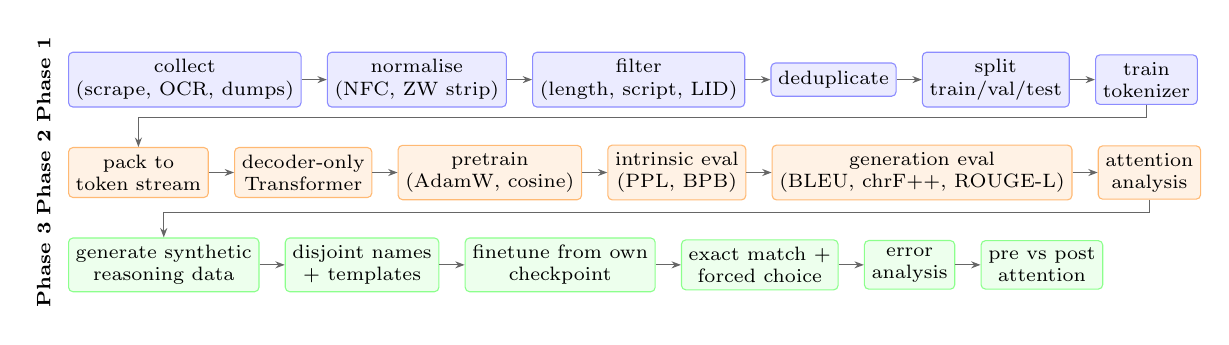
\begin{tikzpicture}[node distance=3.2mm]
\node[hstage] (c1) {collect\\(scrape, OCR, dumps)};
\node[hstage, right=of c1] (c2) {normalise\\(NFC, ZW strip)};
\node[hstage, right=of c2] (c3) {filter\\(length, script, LID)};
\node[hstage, right=of c3] (c4) {deduplicate};
\node[hstage, right=of c4] (c5) {split\\train/val/test};
\node[hstage, right=of c5] (c6) {train\\tokenizer};
\node[lstage, below=5.0mm of c1.south west, anchor=north west] (p1) {pack to\\token stream};
\node[lstage, right=of p1] (p2) {decoder-only\\Transformer};
\node[lstage, right=of p2] (p3) {pretrain\\(AdamW, cosine)};
\node[lstage, right=of p3] (p4) {intrinsic eval\\(PPL, BPB)};
\node[lstage, right=of p4] (p5) {generation eval\\(BLEU, chrF++, ROUGE-L)};
\node[lstage, right=of p5] (p6) {attention\\analysis};
\node[stage, below=5.0mm of p1.south west, anchor=north west, fill=green!7, draw=green!45] (r1) {generate synthetic\\reasoning data};
\node[stage, right=of r1, fill=green!7, draw=green!45] (r2) {disjoint names\\+ templates};
\node[stage, right=of r2, fill=green!7, draw=green!45] (r3) {finetune from own\\checkpoint};
\node[stage, right=of r3, fill=green!7, draw=green!45] (r4) {exact match +\\forced choice};
\node[stage, right=of r4, fill=green!7, draw=green!45] (r5) {error\\analysis};
\node[stage, right=of r5, fill=green!7, draw=green!45] (r6) {pre vs post\\attention};
\foreach \a/\b in {c1/c2, c2/c3, c3/c4, c4/c5, c5/c6, p1/p2, p2/p3, p3/p4, p4/p5, p5/p6,
                   r1/r2, r2/r3, r3/r4, r4/r5, r5/r6}
  \draw[flow] (\a) -- (\b);
\draw[flow] (c6.south) -- ++(0,-1.6mm) -| (p1.north);
\draw[flow] (p6.south) -- ++(0,-1.6mm) -| (r1.north);
\node[font=\scriptsize\bfseries, left=1.0mm of c1, rotate=90, anchor=south] {Phase 1};
\node[font=\scriptsize\bfseries, left=1.0mm of p1, rotate=90, anchor=south] {Phase 2};
\node[font=\scriptsize\bfseries, left=1.0mm of r1, rotate=90, anchor=south] {Phase 3};
\end{tikzpicture}
\caption{The evidence chain, run twice and independently --- once per language. Only
source code is shared. The two vertical arrows carry Phase~1 decisions into later
measurements; Section~\ref{sec:cross} shows that both of them did.}
\label{fig:pipeline}
\end{figure}

\textbf{Contributions.} (i) Two corpora built to the 500M-token target with manual
collection well above the 20\% floor; (ii) a from-scratch Transformer whose causal
mask is verified empirically rather than assumed; (iii) an evaluation that reports
perplexity and bits-per-byte together and shows they disagree; (iv) a reasoning
evaluation with a second metric that contradicts the headline number, reported as
such; (v) two Phase~1 defects traced forward to the measurements they distorted.

\begin{table}[!htb]
\centering\small
\caption{Project setup. The architecture is deliberately identical, so the
non-embedding parameter count matches exactly and model capacity is excluded as an
explanation for any difference in results.}
\label{tab:setup}
\begin{tabular}{lcc}
\toprule
& \textbf{Model H} & \textbf{Model L} \\
\midrule
Language (tier) & Hindi (higher-resource) & Nepali (lower-resource) \\
Script & Devanagari & Devanagari \\
Corpus tokens (train+val+test) & 505{,}852{,}028 & 635{,}204{,}333 \\
Documents & 704{,}101 & 1{,}918{,}265 \\
Manually collected share & 30.66\% & 26.41\% \\
Tokenizer / vocabulary & SentencePiece Unigram / 8{,}000 & SentencePiece BPE / 10{,}000 \\
Total parameters & 23{,}273{,}472 & 24{,}297{,}472 \\
Non-embedding parameters & \textbf{18{,}915{,}328} & \textbf{18{,}915{,}328} \\
Pretraining tokens consumed & 475{,}791{,}360 & 473{,}169{,}920 \\
Evaluated checkpoint & step 14{,}500 & step 14{,}000 \\
\bottomrule
\end{tabular}
\end{table}

% =====================================================================
\section{Phase 1: Corpora and Tokenizers}

\subsection{Sources and manual collection}

Both corpora had to reach roughly 500M tokens with at least 20\% manually collected.
Model~H's manual lane is a Hindi Wikipedia XML dump I downloaded and extracted myself
with WikiExtractor (66.7M tokens), Gadya Kosh prose (59.9M), the patrika.com archive
(19.5M), Kavita Kosh poetry (8.1M) and 15 archive.org items surviving cleaning of 67
collected (0.85M); its downloaded lane is FineWeb-2 \texttt{hin\_Deva} and four
AI4Bharat Sangraha partitions. A HuggingFace mirror of Hindi Wikipedia was quarantined
rather than used, since it duplicates the dump already extracted. Model~L's manual lane
is dominated by an \texttt{onlinekhabar} scrape (91.6\% of its manual tokens), with a
self-parsed Wikipedia dump, BBC Nepali, Wikibooks, Wiktionary, Ekantipur, Ratopati,
Nagarik and OCR of archive.org books; its downloaded lane is AI4Bharat Sangraha and
IndicCorpV2. For Nepali I set absolute targets (100M manual, 400M downloaded) rather
than a percentage and met both at 167.8M and 467.4M. Each site's \texttt{robots.txt}
was checked before scraping and the verdict recorded in
\texttt{scripts/manual\_sites.json}; bhaskar.com and amarujala.com disallow automated
access and were not scraped.

\begin{figure}[!htb]
\centering
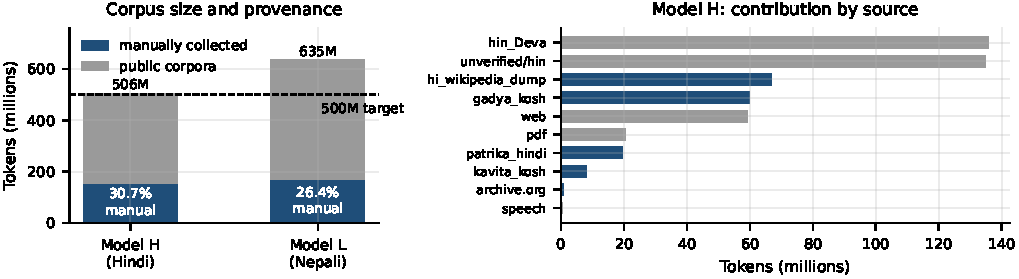
\includegraphics[width=\textwidth]{fig_corpus_composition.pdf}
\caption{Both corpora clear the 500M-token target and the 20\% manual floor. Right:
Model~H's per-source contribution, manual lane in blue --- no single source dominates,
and the manual lane spans five distinct source types.}
\label{fig:composition}
\end{figure}

\subsection{Cleaning, normalisation and deduplication}

Normalisation (\texttt{scripts/clean\_lib.py}) is exactly four operations: NFC
normalise, strip zero-width and C0/C1 control characters, collapse inline whitespace
runs, collapse blank-line runs. ZWNJ and ZWJ are deliberately preserved, because in
Devanagari they change the rendered glyph and are part of the text rather than noise.
NFC matters for a second, less obvious reason: the same Devanagari string has more
than one byte representation, and without normalising first those forms hash
differently and both survive deduplication. A document is then dropped if it is under
200 characters, if fewer than half its characters are Devanagari, if more than 1\% of
it is U+FFFD, or if language identification rejects it. The language verdict is
three-valued --- yes, no, or undetermined --- so a document is not discarded merely
because the detector was unsure. Hindi additionally runs a Bhojpuri lexical reject
filter, needed because Bhojpuri shares both script and much vocabulary with Hindi.

The two pipelines deduplicate differently, and this asymmetry matters later
(Section~\ref{sec:cross}). Model~H uses a SHA-1 hash over punctuation-stripped,
case-folded, whitespace-collapsed text: it removes exact copies and formatting
variants, but by construction cannot detect paraphrase or partial overlap. Model~L
uses exact \texttt{doc\_id} matching followed by MinHash with LSH (100 permutations,
20 bands of 5 rows, 5-character shingles, Jaccard threshold 0.55), and adds a
decontamination stage that removes training documents matching validation or test.

\begin{figure}[!htb]
\centering
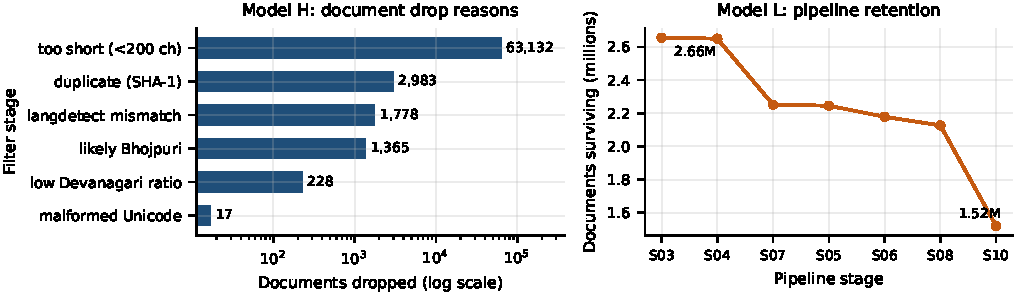
\includegraphics[width=\textwidth]{fig_corpus_funnel.pdf}
\caption{Left: Model~H's drop reasons --- length dominates, and SHA-1 removes only
2{,}983 documents (0.4\%). Right: Model~L's survivor count by stage. S09 is not a
separate point because it records a removal count, not a total: its 17{,}111
decontaminated documents plus S10's 589{,}223 lane-balancing drops account exactly for
the fall from 2.13M to 1.52M.}
\label{fig:funnel}
\end{figure}

\begin{table}[!htb]
\centering\small
\caption{Preprocessing outcomes. The deduplication rows are not comparable
like-for-like: they are the outputs of two different algorithms, which is itself the
finding. Model~H's figure is an exact-duplicate count and says nothing about near
duplicates, which were never measured for Hindi.}
\label{tab:cleaning}
\begin{tabular}{lrr}
\toprule
& \textbf{Model H (Hindi)} & \textbf{Model L (Nepali)} \\
\midrule
Raw documents & 773{,}606 & 2{,}655{,}504 \\
Documents after cleaning & 704{,}103 & 2{,}126{,}334 (post-dedup) \\
Character retention & 95.9\% & --- \\
Dropped: too short ($<$200 chars) & 63{,}132 & --- \\
Dropped: language / script filters & 3{,}371 & 5{,}861 (S04 LID) \\
Deduplication method & SHA-1 exact + formatting & MinHash + LSH (0.55 Jaccard) \\
Duplicates removed & 2{,}983 (exact only) & 2{,}350 exact $+$ 49{,}734 near \\
Train/test decontamination & \textbf{not performed} & 17{,}111 removed, rescan clean \\
Cross-lane duplicates resolved manual-first & --- & 21{,}273 pairs \\
\bottomrule
\end{tabular}
\end{table}

\subsection{Splits and tokenizers}

Both corpora are split by document, never by chunk, so two halves of one article
cannot land on opposite sides of the split and turn memorisation into test accuracy.
Model~H is 96/2/2 (seed 42, shuffle-then-slice), giving 485{,}280{,}741 /
10{,}484{,}640 / 10{,}086{,}647 tokens. Model~L is 85/7.5/7.5 (seed 20260817,
deterministic hash of document id), giving 519{,}906{,}359 / 57{,}839{,}396 /
57{,}458{,}578, and holds validation and test out at stage S07 \emph{before} the
quality filters run, so those filters shape only the training pool and cannot make the
evaluation sets easier. Its \texttt{split\_stats.json} records zero document-id
overlap between splits, and a separate cross-language check found 0 documents shared
between the two corpora.

Both tokenizers were trained from scratch, with vocabulary size chosen by measurement
on held-out text rather than convention. Fertility keeps improving with size for both,
so the choice trades it against the embedding parameters a larger vocabulary costs:
for Model~H, 8{,}000 to 10{,}000 buys less fertility than 5{,}000 to 8{,}000 did and
would spend roughly 1M parameters of a 25M budget, so 8{,}000 was adopted. Model~L
took 10{,}000, the best fertility in its sweep.

\begin{figure}[!htb]
\centering
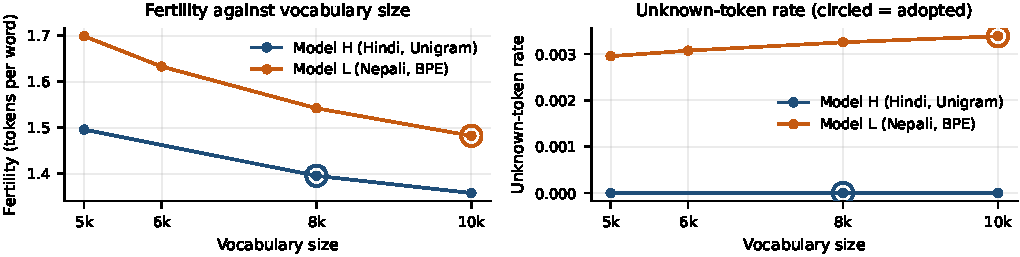
\includegraphics[width=\textwidth]{fig_tokenizer_sweep.pdf}
\caption{The measured sweep; circled points are the adopted sizes. Model~H holds an
unknown rate of exactly zero at every size because its Unigram model has byte
fallback; Model~L's is non-zero everywhere and \emph{rises} with vocabulary size. I
read its byte-fallback column of zeros as a good score. It records that the feature is
absent, and Section~\ref{sec:cross} gives the failure it caused two phases later.}
\label{fig:tokenizer}
\end{figure}


% =====================================================================
\section{Phase 2: Architecture, Pretraining and Evaluation}

\subsection{Implementation}

The model is a decoder-only pre-norm Transformer written with
\texttt{nn.Linear}, \texttt{nn.Embedding}, \texttt{nn.LayerNorm},
\texttt{nn.Dropout} and ordinary tensor operations only. No
\texttt{nn.Transformer*}, no \texttt{nn.MultiheadAttention}, no
\texttt{F.scaled\_dot\_product\_attention} and no HuggingFace model class is used;
a unit test walks the module tree and fails if any of them ever appears, so the
constraint cannot be broken by a later edit.

Inside attention, $W_Q$, $W_K$ and $W_V$ are kept as three separate
\texttt{nn.Linear} layers rather than one fused projection. That is marginally
slower but keeps the three roles visible in the code. Each projection maps
$(B,T,512)$; a \texttt{view} reshapes to $(B,T,8,64)$ and a \texttt{transpose} to
$(B,8,T,64)$, giving eight independent 64-dimensional heads. Scores are
$QK^{\top}/\sqrt{64}$; the scaling is required because dot products of longer vectors
grow in magnitude, and without it the softmax saturates and gradients through it
vanish. The causal mask is built with \texttt{torch.triu(..., diagonal=1)},
registered non-persistently, and applied by \texttt{masked\_fill} with $-\infty$
before the softmax.

\textbf{Causal masking, verified rather than assumed.} The test in
\texttt{tests/test\_model.py} perturbs every token after position $t$ and measures
the largest change in the logits at positions $\le t$. It is exactly
$0.000\mathrm{e}{+}00$ --- not merely small, because $\mathrm{softmax}(-\infty)$ is
exactly zero and contributes exactly nothing. The same test asserts the converse,
that outputs at the perturbed positions \emph{do} change; without that check a model
that ignored its input entirely would also pass. Both language suites pass 9/9.

\begin{figure}[!htb]
\centering
\begin{minipage}[c]{0.40\textwidth}
\centering
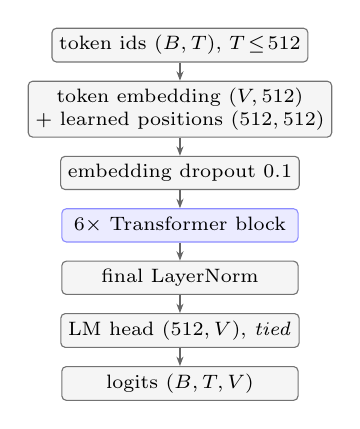
\begin{tikzpicture}[node distance=2.3mm, every node/.style={font=\scriptsize}]
\node[stage, minimum width=30mm] (ids) {token ids $(B,T)$, $T\!\le\!512$};
\node[stage, below=of ids, minimum width=30mm] (emb) {token embedding $(V,512)$\\$+$ learned positions $(512,512)$};
\node[stage, below=of emb, minimum width=30mm] (drop) {embedding dropout $0.1$};
\node[hstage, below=of drop, minimum width=30mm] (blk) {$6\times$ Transformer block};
\node[stage, below=of blk, minimum width=30mm] (ln) {final LayerNorm};
\node[stage, below=of ln, minimum width=30mm] (head) {LM head $(512,V)$, \emph{tied}};
\node[stage, below=of head, minimum width=30mm] (log) {logits $(B,T,V)$};
\foreach \a/\b in {ids/emb, emb/drop, drop/blk, blk/ln, ln/head, head/log}
  \draw[flow] (\a) -- (\b);
\end{tikzpicture}
\end{minipage}\hfill
\begin{minipage}[c]{0.27\textwidth}
\centering
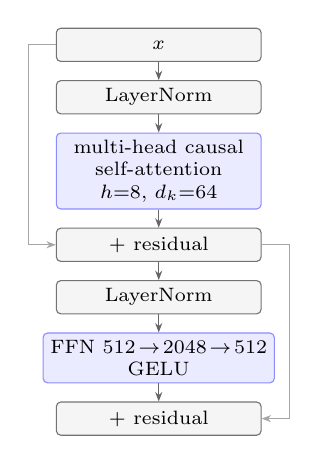
\begin{tikzpicture}[node distance=2.3mm, every node/.style={font=\scriptsize}]
\node[stage, minimum width=26mm] (x) {$x$};
\node[stage, below=of x, minimum width=26mm] (n1) {LayerNorm};
\node[hstage, below=of n1, minimum width=26mm] (at) {multi-head causal\\self-attention\\$h{=}8$, $d_k{=}64$};
\node[stage, below=of at, minimum width=26mm] (a1) {$+$ residual};
\node[stage, below=of a1, minimum width=26mm] (n2) {LayerNorm};
\node[hstage, below=of n2, minimum width=26mm] (ff) {FFN $512\!\to\!2048\!\to\!512$\\GELU};
\node[stage, below=of ff, minimum width=26mm] (a2) {$+$ residual};
\foreach \a/\b in {x/n1, n1/at, at/a1, a1/n2, n2/ff, ff/a2}
  \draw[flow] (\a) -- (\b);
\draw[flow, draw=black!35] (x.west) -- ++(-3.5mm,0) |- (a1.west);
\draw[flow, draw=black!35] (a1.east) -- ++(3.5mm,0) |- (a2.east);
\end{tikzpicture}
\end{minipage}\hfill
\begin{minipage}[c]{0.30\textwidth}
\centering\scriptsize
\captionsetup{type=table}
\captionof{table}{Parameter breakdown, derived from the configuration and asserted
against the loaded model.}
\label{tab:params}
\begin{tabular}{lrr}
\toprule
& \textbf{H} & \textbf{L} \\
\midrule
Token emb.\ $V{\times}512$ & 4.10M & 5.12M \\
Positions $512{\times}512$ & 0.26M & 0.26M \\
Attention $4{\times}6$ proj. & 6.30M & 6.30M \\
Feed-forward $6{\times}$ & 12.60M & 12.60M \\
LayerNorms & 0.01M & 0.01M \\
LM head (tied) & 0 & 0 \\
\midrule
Non-embedding & 18.92M & 18.92M \\
\textbf{Total} & \textbf{23.27M} & \textbf{24.30M} \\
\bottomrule
\end{tabular}
\end{minipage}
\caption{Forward pass, one pre-norm block expanded, and where the parameters sit, at
the configuration actually trained. Weight tying removes a second $V\!\times\!512$
matrix, saving 4{,}096{,}000 parameters for Model~H ($\approx$15\%). Six blocks of
3{,}152{,}384 plus a final LayerNorm give 18{,}915{,}328 non-embedding parameters; a
seventh would overshoot 25M.}
\label{fig:arch}
\end{figure}

\textbf{Design choices.} Depth was preferred over width: each block costs
3.15M parameters, so six blocks plus embeddings land at 23.27M where seven would
reach 26.4M, and attention needs several rounds of composition to build multi-step
dependencies. Positions are learned and absolute, chosen because the model is trained
and evaluated at one fixed length where the extrapolation advantage of sinusoidal
encodings does not apply; the price is that 512 is a hard ceiling, since no embedding
row exists for position 512. Pre-norm was used for gradient stability through the
stack. Dropout at 0.1 is applied in four places: attention probabilities, attention
output, feed-forward output and the embedding sum.

\subsection{Pretraining}

\begin{table}[!htb]
\centering\small
\caption{Training configuration, identical for both models apart from vocabulary
size. Both runs were stopped by an 11-hour wall-clock guard placed in the trainer so
that a dying Kaggle session could never leave an unusable state.}
\label{tab:train}
\begin{tabular}{llll}
\toprule
Optimiser & AdamW, $\beta=(0.9,\,0.95)$ & Effective batch & $32\times2\times512 = 32{,}768$ tokens \\
Weight decay & 0.1, matrices only ($\dim\ge2$) & Precision & bfloat16 \\
Peak / min LR & $6{\times}10^{-4}$ / $6{\times}10^{-5}$ & Hardware & Kaggle Tesla T4 \\
Schedule & 500 warmup, then cosine & Throughput & 12{,}024 / 11{,}958 tok\,s$^{-1}$ \\
Gradient clipping & 1.0, after \texttt{unscale\_} & Wall clock & 10.99 h each \\
Seed & 20260902 & Steps reached & 14{,}520 / 14{,}440 of 15{,}000 \\
\bottomrule
\end{tabular}
\end{table}

Every checkpoint carries model weights, optimizer state, scheduler state, training
step, best validation loss, tokens consumed, both RNG states and the full
configuration, so an interrupted session resumes exactly rather than approximately.
I verified resume across three deliberately killed sessions before starting the real
runs. Checkpoints are written on best validation loss, so the evaluated checkpoints
are step 14{,}500 (H) and 14{,}000 (L).

Neither run finished its planned 15{,}000 steps. The wall-clock guard fired first,
costing about 3\% of the token budget, and both validation curves
(Figure~\ref{fig:curves}) are still descending at the last checkpoint. Neither model
is converged, and the absolute perplexities below should be read with that in mind;
the comparison between them is unaffected because both stopped under the same rule
with near-identical token budgets.

\begin{figure}[!htb]
\centering
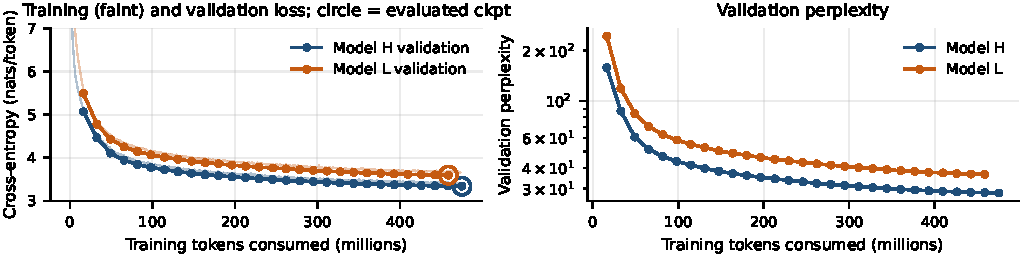
\includegraphics[width=\textwidth]{fig_pretrain_curves.pdf}
\caption{Both validation curves are still falling when the wall-clock guard stops the
run, so neither model is converged. The gap between them is stable from roughly 150M
tokens onward, which is what keeps the comparison meaningful anyway.}
\label{fig:curves}
\end{figure}

\subsection{Intrinsic evaluation: two metrics that disagree}

\begin{table}[!htb]
\centering\small
\caption{Intrinsic metrics on each model's own test split, scored over an identical
budget of 1{,}999{,}872 tokens per model.}
\label{tab:intrinsic}
\begin{tabular}{lrr@{\hskip 20pt}lrr}
\toprule
& \textbf{Model H} & \textbf{Model L} & & \textbf{Model H} & \textbf{Model L} \\
\midrule
Cross-entropy (nats) & 3.3109 & 3.8433 & Bytes per token & 8.875 & 11.441 \\
Test perplexity & \textbf{27.41} & 46.68 & Bytes scored & 17{,}749{,}798 & 22{,}880{,}653 \\
Bits per token & 4.7766 & 5.5447 & \textbf{Test bits-per-byte} & 0.5382 & \textbf{0.4846} \\
\bottomrule
\end{tabular}
\end{table}

Perplexity says Model~H is 41\% better. Bits-per-byte says Model~L is slightly
better. Both are correct, because they measure per different units. Perplexity is per
token, and a token is not the same quantity of text in the two models: Model~L's BPE
holds 11.44 bytes where Model~H's Unigram holds 8.88. Model~L's tokens are
individually harder to predict, but each one carries about 29\% more text. Dividing
by bytes removes the tokenizer from the comparison, and when it is removed the
ordering reverses.

\textbf{Interpretation and its limit.} The right reading is that most of the apparent
perplexity gap is tokenizer granularity rather than model quality. It does
\emph{not} follow that Model~L is the better language model: bits-per-byte is a
tokenizer-neutral measure but not a corpus-neutral one, and the two models are scored
on different text of different intrinsic difficulty. Model~L's corpus is nominally
larger but 91.6\% of its manual lane is a single news source, so it may simply be
more predictable text. Separating those two explanations would need a parallel or
translated evaluation set, which this project does not have.

\begin{figure}[!htb]
\centering
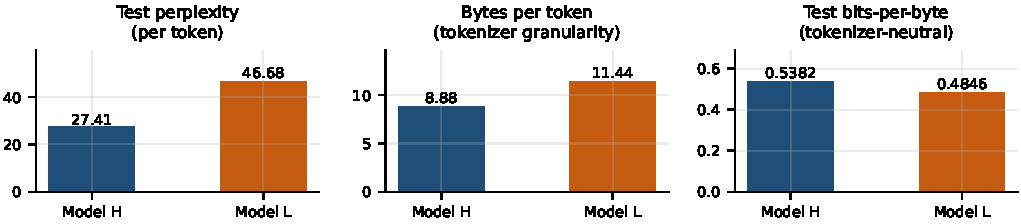
\includegraphics[width=\textwidth]{fig_ppl_bpb.pdf}
\caption{The reversal. The middle panel is the mechanism --- not a quality measure but
a property of the tokenizers, large enough to flip the ordering between the outer two.
Reporting only the left panel would have supported a conclusion the right panel does
not support.}
\label{fig:pplbpb}
\end{figure}

\subsection{Generation}

Continuations were generated from 64 held-out prefixes of 64 tokens each, continued
for 64 tokens, under greedy decoding and temperatures 0.5, 1.0 and 1.5, and scored
against the true continuations.

\begin{table}[!htb]
\centering\small
\caption{Generation metrics across all four decoding settings. BLEU is corpus-level
BLEU-4 (sacreBLEU); chrF++ uses character 6-grams plus word 2-grams; repetition is
the fraction of repeated 4-grams.}
\label{tab:generation}
\begin{tabular}{llrrrrrr}
\toprule
& & \multicolumn{3}{c}{\textbf{Overlap with reference}} & \multicolumn{3}{c}{\textbf{Fluency / diversity}} \\
\cmidrule(lr){3-5}\cmidrule(lr){6-8}
Model & Decoding & BLEU-4 & chrF++ & ROUGE-L & Repetition & Distinct-1 & Distinct-2 \\
\midrule
H & greedy  & 1.96 & 12.49 & 0.093 & 0.598 & 0.172 & 0.313 \\
H & $T=0.5$ & 1.80 & 14.33 & 0.096 & 0.212 & 0.275 & 0.602 \\
H & $T=1.0$ & 1.01 & \textbf{16.29} & \textbf{0.100} & 0.002 & 0.520 & 0.939 \\
H & $T=1.5$ & 0.16 & 14.67 & 0.053 & 0.000 & 0.702 & 0.992 \\
\midrule
L & greedy  & 2.37 & 14.48 & 0.081 & 0.577 & 0.179 & 0.263 \\
L & $T=0.5$ & 1.88 & 16.54 & \textbf{0.092} & 0.190 & 0.345 & 0.611 \\
L & $T=1.0$ & 1.69 & \textbf{18.05} & 0.079 & 0.001 & 0.634 & 0.948 \\
L & $T=1.5$ & 0.78 & 16.13 & 0.035 & 0.000 & 0.793 & 0.995 \\
\bottomrule
\end{tabular}
\end{table}

Greedy decoding degenerates in both models: roughly 58--60\% of its 4-grams are
repeats and the text visibly loops. That is not a defect in the models but a property
of the decoding rule --- greedy always takes the argmax, so once the model re-enters
a state it has visited it reproduces the same continuation with no escape. Temperature
1.0 removes the repetition and simultaneously gives the best chrF++ for both models,
so on these models additional diversity cost nothing in overlap quality.

BLEU sits near the floor everywhere and is not informative here: an open-ended
continuation has no particular reason to share 4-grams with a single reference, and
the estimate is correspondingly noisy. chrF++ is the metric I would defend for this
pair, because character $n$-grams survive the morphology --- in Devanagari a single
changed suffix destroys a whole-word match but leaves most character $n$-grams intact.
ROUGE-L is computed over whitespace tokens, which under-segment Devanagari, making it
the least reliable of the three. All three are reported because the specification
requires them, not because all three are equally meaningful.

\begin{figure}[!htb]
\centering
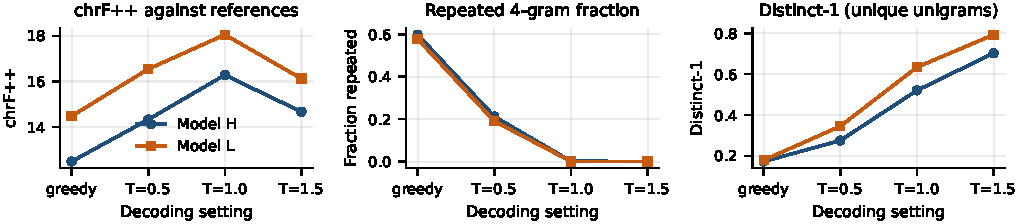
\includegraphics[width=\textwidth]{fig_decoding_sweep.pdf}
\caption{Quality peaks at $T=1.0$ while repetition has already collapsed to near zero,
so the usual quality--diversity trade-off does not bind in this range. Model~L is
consistently higher on both, consistent with its coarser tokens covering more text per
generated step.}
\label{fig:decoding}
\end{figure}

\subsection{Attention analysis}

Mean attention entropy is 3.2047 nats for Model~H and 3.0898 for Model~L against a
uniform baseline of 5.2565 for the same sequence length; the baseline is computed
rather than assumed, because an entropy of 3.2 means nothing without it. Mean
attention distance is 62.36 and 54.51 token positions.

\begin{figure}[!htb]
\centering
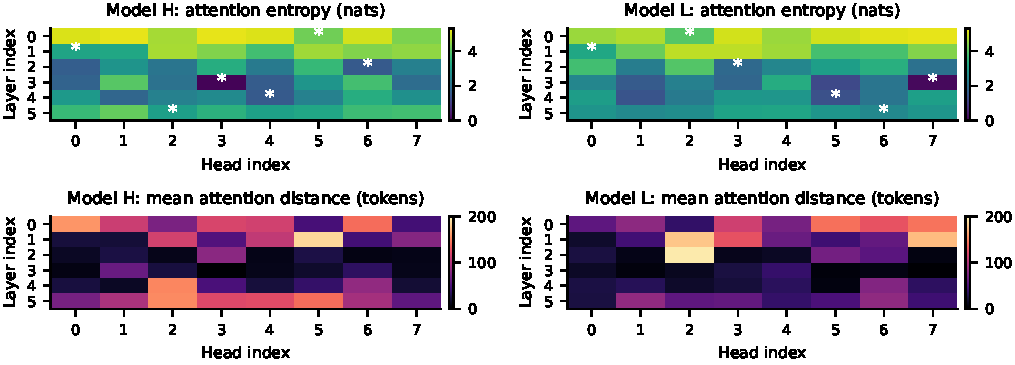
\includegraphics[width=\textwidth]{fig_attention_grid.pdf}
\caption{Every head of every layer; the asterisk marks each layer's sharpest head.
Both models independently develop a near-deterministic previous-token head at layer~3
(entropy 0.06 at distance 1.3 for H; 0.14 at 1.1 for L) despite different languages,
tokenizers and seeds, with attention diffuse at layer~0, sharpening to layer~3 and
broadening by layer~5. This is a consistent pattern, not evidence of a functional
role.}
\label{fig:attngrid}
\end{figure}

\begin{figure}[!htb]
\centering
\begin{subfigure}{0.49\textwidth}
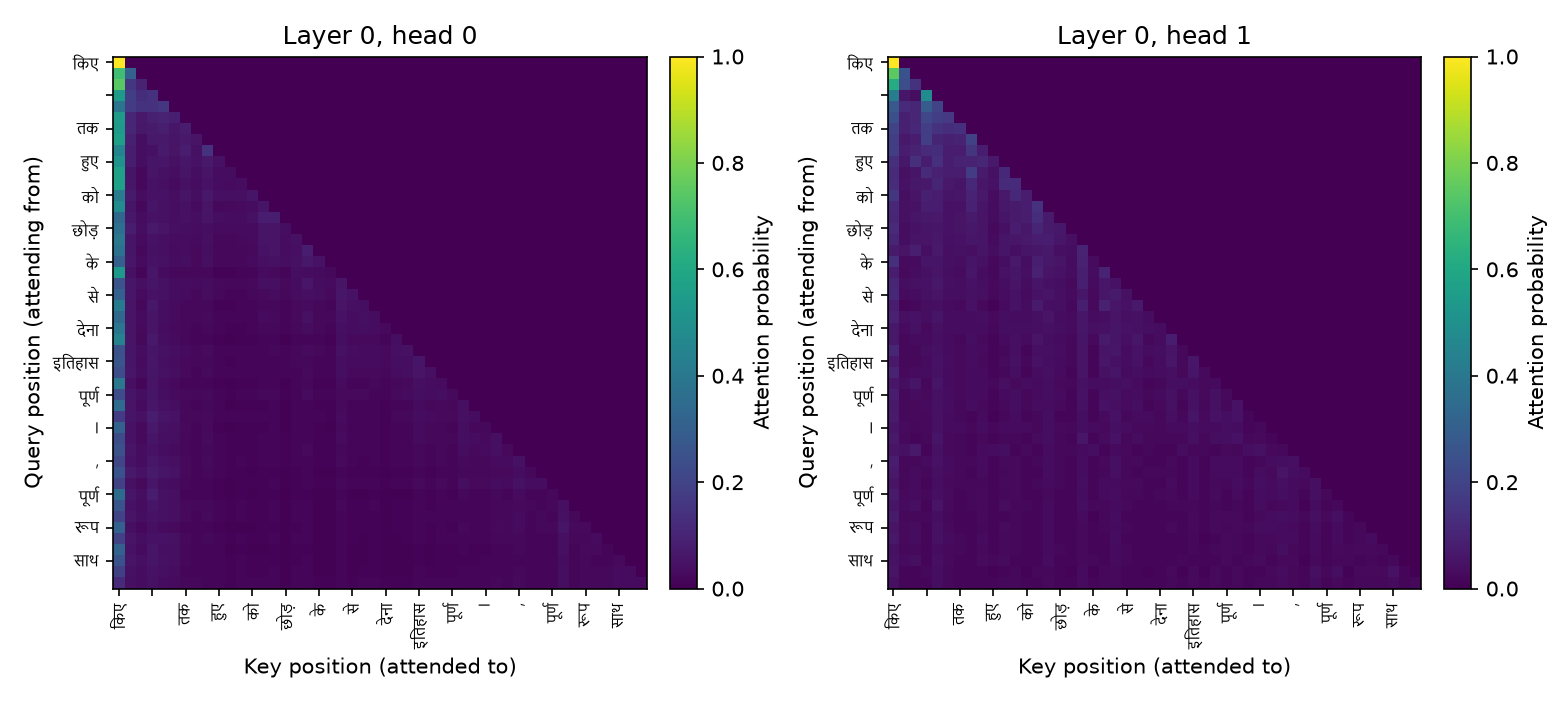
\includegraphics[width=\textwidth]{crop_hindi_attention_layer0.png}
\caption{Model~H, layer 0}
\end{subfigure}\hfill
\begin{subfigure}{0.49\textwidth}
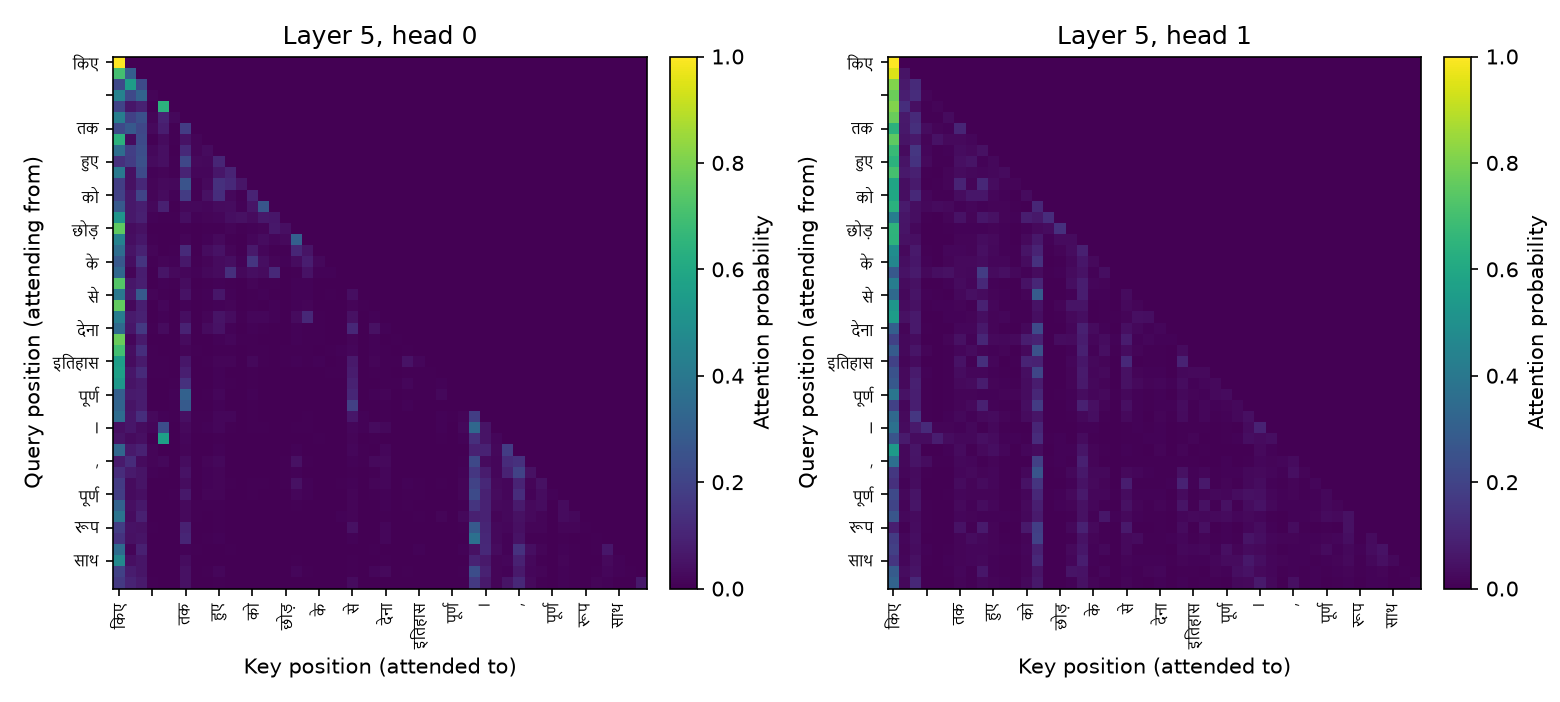
\includegraphics[width=\textwidth]{crop_hindi_attention_layer5.png}
\caption{Model~H, layer 5}
\end{subfigure}
\caption{Causal self-attention on a held-out Hindi sentence, showing the first two
heads of an early and a late layer. Layer~0 is broad and position-driven; layer~5
shows narrow vertical stripes --- many queries concentrating on the same few keys
regardless of position, which is content-driven rather than positional. All four
heads per layer, and the Nepali equivalents, are in \texttt{report/phase2/figures/}.}
\label{fig:heatmaps}
\end{figure}

% =====================================================================
\section{Phase 3: Reasoning Finetuning}

\subsection{Synthetic dataset}

Rather than download a benchmark, I wrote a generator per language so that the
ground-truth answer is known by construction and the train/test relationship is fully
controlled. Four task families are produced in equal proportion: \texttt{compare2}
(one-step comparison between two entities), \texttt{numeric2} and \texttt{numeric3}
(comparison over explicit quantities for two or three entities), and
\texttt{transitive3} (a two-hop chain, $A \mathbin{R} B$ and $B \mathbin{R} C$, asking
for an extreme). Each language gets 20{,}000 training, 2{,}000 validation and 2{,}000
test examples. The Hindi and Nepali sets share no sentence, no entity name and no
template.

\begin{figure}[!htb]
\centering
\begin{minipage}[c]{0.63\textwidth}
\centering
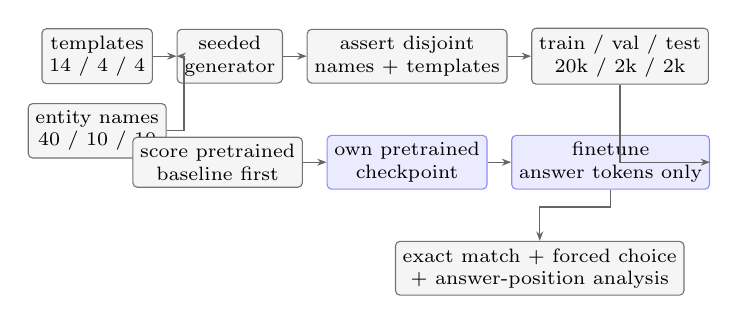
\begin{tikzpicture}[node distance=3.0mm, every node/.style={font=\scriptsize}]
\node[stage] (t) {templates\\14 / 4 / 4};
\node[stage, below=2.4mm of t] (n) {entity names\\40 / 10 / 10};
\node[stage, right=of t] (g) {seeded\\generator};
\node[stage, right=of g] (a) {assert disjoint\\names + templates};
\node[stage, right=of a] (s) {train / val / test\\20k / 2k / 2k};
\node[hstage, below=6.5mm of a] (ck) {own pretrained\\checkpoint};
\node[hstage, right=of ck] (ft) {finetune\\answer tokens only};
\node[stage, left=of ck] (sc) {score pretrained\\baseline first};
\node[stage, below=6.5mm of ft, xshift=-9mm] (ev) {exact match $+$ forced choice\\$+$ answer-position analysis};
\draw[flow] (t) -- (g); \draw[flow] (n.east) -- ++(2.2mm,0) |- (g.west);
\draw[flow] (g) -- (a); \draw[flow] (a) -- (s);
\draw[flow] (s.south) |- (ft.east);
\draw[flow] (sc) -- (ck); \draw[flow] (ck) -- (ft);
\draw[flow] (ft.south) -- ++(0,-2.2mm) -| (ev.north);
\end{tikzpicture}
\end{minipage}\hfill
\begin{minipage}[c]{0.35\textwidth}
\centering\scriptsize
\captionsetup{type=table}
\captionof{table}{Reasoning dataset, per language.}
\label{tab:reasondata}
\begin{tabular}{lr}
\toprule
Train / val / test & 20{,}000 / 2{,}000 / 2{,}000 \\
Task families & 4, 5{,}000 train each \\
Templates (tr/va/te) & 14 / 4 / 4 \\
Entity names & 40 / 10 / 10 \\
Names disjoint & asserted true \\
Templates disjoint & asserted true \\
Distinct train prompts & 20{,}000 \\
Mean prompt length & 71.1 chars (H) \\
\bottomrule
\end{tabular}
\end{minipage}
\caption{Generation and finetuning pipeline. Leakage is controlled on two axes at once:
a test question concerns people the model has never seen, phrased in a way it has never
seen. Both properties are asserted inside the generator, not assumed. Scoring the
pretrained baseline \emph{before} finetuning is a sequencing constraint --- once the
weights change, that number is unrecoverable without retraining.}
\label{fig:reasonpipe}
\end{figure}

\textbf{Two defects found during construction.} Both would have invalidated the
results had they survived.
\begin{itemize}
\item \emph{Gender-agreement leak.} Hindi adjectives inflect for gender, so a question
such as ``who is smallest?'' asked about one woman and two men has only one
grammatically well-formed answer --- solvable without comparing anything. 181 of 400
sampled examples were answerable that way. Detected by inspecting generated examples
for a shortcut; fixed by drawing all entities in an example from one gender.
\item \emph{Nepali numerals.} The Nepali BPE vocabulary
contains no Devanagari digit at all --- not one of \dn{०--९} --- and, having no byte
fallback, mapped every number in the generated data to \texttt{<unk>}: 4.8\% of the
corpus. Detected by tokenizing the generated set and checking its unknown rate before
training. Fixed by switching Nepali numerals to Arabic digits, which the vocabulary
covers completely and which modern Nepali writing uses anyway. Both sets now tokenize
at exactly zero unknowns.
\end{itemize}

\subsection{Protocol and metrics}

Each model is finetuned from its own pretrained checkpoint with its own tokenizer
held fixed; the finetuning script asserts that the tokenizer vocabulary size matches
the checkpoint rather than trusting the configuration file. Loss is computed on answer
tokens only (\texttt{ignore\_index=-1} over the prompt), so the model earns no credit
for reproducing question text. Batches are grouped by length instead of padded ---
necessary rather than cosmetic, because with learned absolute positions any left
padding would shift the position index of every real token. Settings: 2 epochs,
batch 32, peak LR $6{\times}10^{-5}$ (one tenth of pretraining, because a
pretraining-sized step overwrites the language model before the task is learned),
100 warmup steps, evaluation every 20 steps, seed 20260914, float16 with a
\texttt{GradScaler} (the T4 is compute capability 7.5 and has no bfloat16).

Two accuracy metrics are reported because neither suffices alone. \emph{Exact match}
after greedy decoding is the honest end-to-end result, but it is pinned at zero for a
model that has never seen this prompt format, so it cannot distinguish ``learned
nothing'' from ``knows the answer but not how to say it''. \emph{Forced choice}
restricts the model to the entity names the question actually contains and picks the
one with the highest length-normalised mean log-probability; its chance rate is
computed per example from the number of candidates and averages 41.67\%.

\subsection{Results}

\begin{table}[!htb]
\centering\small
\caption{Pretrained versus finetuned on 2{,}000 held-out test questions per model,
with unseen names and unseen templates. The exact-match column rises sharply; the
forced-choice column does not move away from chance in either model.}
\label{tab:reasoning}
\begin{tabular}{lrrr@{\hskip 20pt}rrr}
\toprule
& \multicolumn{3}{c}{\textbf{Model H}} & \multicolumn{3}{c}{\textbf{Model L}} \\
\cmidrule(lr){2-4}\cmidrule(lr){5-7}
& pretrained & finetuned & $\Delta$ & pretrained & finetuned & $\Delta$ \\
\midrule
Exact match & 0.00\% & 35.15\% & $+35.15$ & 0.00\% & 29.45\% & $+29.45$ \\
Forced choice (chance 41.67\%) & 39.80\% & 36.35\% & $-3.45$ & 38.80\% & 39.30\% & $+0.50$ \\
Answer-token loss (nats) & 5.2439 & 0.9408 & $-4.3031$ & 5.5367 & 1.4351 & $-4.1016$ \\
Answer-token perplexity & 189.40 & 2.56 & --- & 253.84 & 4.20 & --- \\
\bottomrule
\end{tabular}
\end{table}

\textbf{Observation.} Exact match rises from zero to 35.15\% and 29.45\%, and
answer-token loss falls by more than four nats in both models.
\textbf{Interpretation.} Finetuning taught the models to emit a candidate name in the
expected position and format; the loss collapse is consistent with that and with
nothing stronger. \textbf{What it does not show.} Under forced choice both models sit
at or below the 41.67\% chance rate, and per task the scores land close to their
individual chance rates --- Model~H reaches 50.40\% and 47.00\% on the two-candidate
families (chance 50\%) and 33.20\% on the three-candidate one (chance 33.3\%). The
result therefore does not establish that either model learned the comparison
operation. The one family that departs from chance departs downward, which is the
subject of the next section.

\begin{figure}[!htb]
\centering
\begin{minipage}{0.375\textwidth}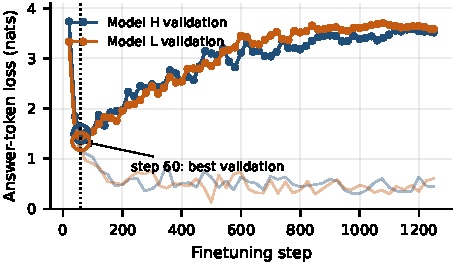
\includegraphics[width=\textwidth]{fig_finetune_curves.pdf}\end{minipage}\hfill
\begin{minipage}{0.605\textwidth}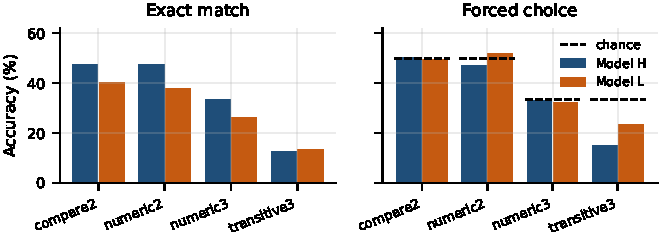
\includegraphics[width=\textwidth]{fig_reasoning_accuracy.pdf}\end{minipage}
\caption{Left: validation loss bottoms out at step~60 while training loss falls to
0.4441 and 0.6048 --- with 40 names and 14 templates, memorising the answer prior is
easier than reading the question. Best-validation checkpointing means the evaluated
models are step~60, so this overfitting never reached the reported numbers. Right:
under forced choice every family sits near its own chance line except
\texttt{transitive3}, which falls well below it in both models.}
\label{fig:phase3results}
\end{figure}

\subsection{Error analysis}

Accuracy alone cannot separate uniform guessing from a positional habit, so the
evaluation records which prompt position each answer came from alongside where the
gold answer actually sits.

\begin{table}[!htb]
\centering\small
\caption{Answer-position distribution on \texttt{transitive3} (finetuned). The chain
is stated as $A \mathbin{R} B$, $B \mathbin{R} C$, so the extremes are always $A$ and
$C$ and the middle entity is \emph{never} correct --- yet it attracts most of
Model~H's answers.}
\label{tab:errors}
\begin{tabular}{lrrrr}
\toprule
& answered $A$ (first) & answered $B$ (middle) & answered $C$ (last) & off-prompt \\
\midrule
Gold distribution & 47.4\% & \textbf{0.0\%} & 52.6\% & --- \\
Model H & \textbf{0.0\%} & \textbf{72.6\%} & 25.4\% & 2.0\% \\
Model L & 3.2\% & 41.8\% & 26.2\% & 28.8\% \\
\bottomrule
\end{tabular}
\end{table}

Model~H selects the middle entity in 72.6\% of two-hop questions and the first entity
in none. $B$ is the only name mentioned twice, so the behaviour is consistent with
selection by surface salience rather than by following the inequality --- and it
explains why this family scores \emph{below} chance, since uniform guessing would at
least hit $A$ and $C$ sometimes. On the one-hop families Model~H prefers the
second-named entity roughly two to one (62.0\% and 65.0\%) against a balanced gold
split, a recency effect:

\begin{quote}\small
\dn{ध्यान दीजिए: नवीन वरुण से अमीर है। अमीर कौन है?} $\rightarrow$ \dn{वरुण}
\;(gold \dn{नवीन}) \hfill
\dn{ध्यान दीजिए: प्रवीण वरुण से हल्का है। भारी कौन है?} $\rightarrow$ \dn{वरुण} \;\checkmark
\end{quote}

The second example requires flipping the direction of the comparison and is answered
correctly; given the positional habit above, such cases are best read as the habit
coinciding with the right answer rather than as evidence of comparison.

The clearest resource-tier difference in the whole project is groundedness. Model~L
answers with a name the question never mentions in 19.2--28.8\% of cases, repeatedly
emitting memorised \emph{training} names (\dn{सिर्जना}, \dn{निरु}); Model~H does so in
0.0--7.2\%. Before finetuning both models do this essentially 100\% of the time, so
finetuning moved Model~H almost entirely onto the prompt and Model~L only about three
quarters of the way.

\begin{figure}[!htb]
\centering
\begin{minipage}{0.355\textwidth}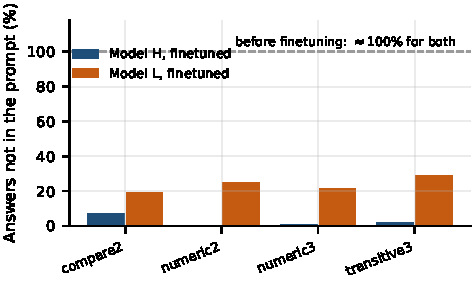
\includegraphics[width=\textwidth]{fig_offprompt.pdf}\end{minipage}\hfill
\begin{minipage}{0.625\textwidth}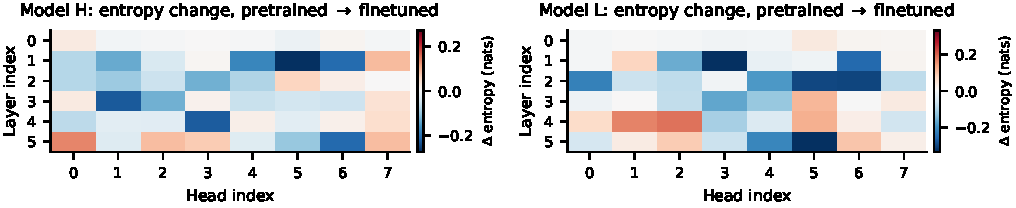
\includegraphics[width=\textwidth]{fig_head_delta.pdf}\end{minipage}
\caption{Left: how often each finetuned model answers with a name absent from the
prompt. Right: per-head entropy change, pretrained to finetuned, on identical held-out
prompts of identical length. Most heads barely move; the largest shifts concentrate in
the middle layers, where Phase~2 located the previous-token heads. This identifies
which heads changed, not what they compute.}
\label{fig:phase3attn}
\end{figure}

\subsection{Attention before and after finetuning}

Both checkpoints were run on the same held-out reasoning prompts, all of identical
token length, so that neither prompt content nor sequence length could masquerade as
a finetuning effect.

\begin{table}[!htb]
\centering\small
\caption{Attention summary on reasoning prompts, pretrained versus finetuned.}
\label{tab:attncompare}
\begin{tabular}{llrrr}
\toprule
Model & Checkpoint & Mean entropy (nats) & Mean distance (tokens) & Uniform baseline \\
\midrule
H & pretrained (step 14{,}500) & 1.9102 & 10.303 & 2.9545 (length 46) \\
H & finetuned (step 60) & 1.8691 & 10.360 & \\
L & pretrained (step 14{,}000) & 1.8327 & 9.415 & 2.8061 (length 39) \\
L & finetuned (step 60) & 1.7833 & 10.157 & \\
\bottomrule
\end{tabular}
\end{table}

Finetuning made attention slightly sharper and slightly longer-range at the same time
in both models, most visibly in Model~L, where mean distance rises 0.74 positions on a
39-token prompt. This is consistent with a shift toward attending to the entity names
scattered across the prompt rather than to local context, but the measurement cannot
establish that: showing that these heads perform the comparison would require
ablating a head and re-scoring, which I did not run. Layer~0 and layer~5 heatmaps for
both checkpoints and both models are in \texttt{report/phase3/figures/}.

% =====================================================================
\section{Cross-Phase Analysis}
\label{sec:cross}

\textbf{Tokenizer $\rightarrow$ intrinsic metrics.} The Phase~1 vocabulary choice
propagates directly into the Phase~2 headline. Model~L's BPE at 10{,}000 produces
11.44 bytes per token against Model~H's 8.88, and that single property is large
enough to reverse the ranking between perplexity and bits-per-byte
(Figure~\ref{fig:pplbpb}). Any cross-language perplexity comparison in this project
is therefore a statement about tokenizers at least as much as about models.

\textbf{Missing byte fallback $\rightarrow$ Phase~3 data corruption.} Model~L's
tokenizer has no byte fallback at any vocabulary size, which in Phase~1 appeared only
as a column of zeros that I read as a good result. It surfaced in Phase~2 as a
0.17--0.34\% unknown-token rate, and in Phase~3 as outright corruption: no Devanagari
digit exists in the vocabulary, so 4.8\% of the generated reasoning corpus became
\texttt{<unk>} before I caught it. One Phase~1 configuration flag, invisible for two
phases, then responsible for a data defect.

\textbf{Deduplication asymmetry $\rightarrow$ a limit on the comparison.} Model~L has
MinHash near-duplicate removal and a train-vs-evaluation decontamination stage;
Model~H has neither, only SHA-1 exact matching, and removed just 2{,}983 documents
(0.4\%) against Model~L's $\approx$52{,}000. Model~H's test split may therefore
overlap its training data in ways Model~L's cannot. This is a genuine confound in the
direction that \emph{flatters} Model~H, and it is not quantified anywhere in this
project; the perplexity gap attributed above to tokenizer granularity and corpus
composition may also contain an unmeasured leakage component. Measuring it would mean
running the Nepali MinHash decontamination over the Hindi corpus, which I did not do.

\textbf{Pretraining $\rightarrow$ reasoning.} The resource tier shows up in Phase~3
not as accuracy but as groundedness. Both models are at chance on the comparison
itself, so pretraining quality did not buy reasoning. What it bought is attention to
the prompt: Model~H answers from the given candidates 93--100\% of the time against
Model~L's 71--81\%. The better-pretrained model is better at \emph{using the input},
which is a weaker and more defensible claim than better reasoning.

\textbf{A measurement artefact worth recording.}
\label{sec:tokencounts}
Phase~1 and Phase~2 report different token counts for the same splits --- 485{,}280{,}741
against 485{,}956{,}678 for Hindi train. The difference is exactly 675{,}937, the
number of documents in that split, because packing appends one end-of-document token
per document. The same identity holds for all six splits (Nepali train differs by
exactly 1{,}520{,}000, its document count). Both numbers are correct for what they
measure; this report uses Phase~1 counts for corpus statistics and packed counts for
the training stream.

% =====================================================================
\section{Limitations, Failures and Lessons}

\begin{itemize}
\item \textbf{Checkpoint-selection grid (detected, fixed, re-run).} The first
finetuning run evaluated every 100 steps and selected its best checkpoint at step
100 --- exactly where warmup ends --- with validation loss rising monotonically
afterwards, so the grid was too coarse to locate the real optimum. Moving to a
20-step grid with nothing else changed raised Model~L from 14.90\% to 29.45\% exact
match and Model~H from 32.70\% to 35.15\%. The superseded run is kept in
\texttt{report/phase3/run\_a\_40names/}.
\item \textbf{Neither pretraining run converged.} Both stopped at the 11-hour guard,
roughly 3\% short of the planned token budget, with validation loss still falling.
Absolute perplexities are therefore upper bounds.
\item \textbf{Hindi deduplication is weaker than Nepali's}, and no decontamination was
run for Hindi. This is the first thing I would fix, and it is a stated limit on the
central comparison rather than a cosmetic gap.
\item \textbf{The reasoning training distribution is too narrow in two ways.} 40 entity
names make the answer prior cheap to memorise, and every example of a given template
is identical apart from slot fillers, so the surface form carries almost no entropy.
Both models overfit by step 60. More entities and per-template linguistic variation
(synonym substitution, clause reordering) are the two independent fixes; the generator
has no variation layer today.
\item \textbf{Attention analysis is correlational.} It identifies which heads changed
and how sharply they attend. It does not establish what any head computes, and no
causal probe (head ablation and re-scoring) was run.
\item \textbf{Manual-share methodology differs between languages} --- Hindi's share is
character-weighted over the cleaned corpus, Nepali's is token-weighted --- so the two
percentages are not strictly like-for-like.
\item \textbf{Lesson.} The same mistake was available twice in opposite directions:
perplexity alone would have overstated the resource gap, and exact match alone would
have overstated the reasoning gain. In both cases a second metric measuring the same
thing in different units was what exposed it. A single headline number was wrong both
times.
\end{itemize}

\textbf{Reproducibility.} Seeds are fixed and recorded at every stage (splits 42 and
20260817; pretraining 20260902; finetuning 20260914). Model, training and finetuning
configurations are YAML files committed beside the code, and the architecture used for
finetuning is read out of the checkpoint rather than from a config file, so a mismatch
is impossible by construction. Checkpoints carry weights, optimizer, scheduler, step,
best validation loss, tokens seen, RNG states and configuration. Every number in this
report is produced by \texttt{scripts/make\_numbers\_sheet.py} reading the result
artifacts, and every figure by \texttt{report/final/make\_final\_figures.py} reading
the same files; neither is hand-entered.

% =====================================================================
\section{Conclusion}

Two independent $\approx$23M-parameter decoder-only Transformers were built from
scratch and trained on self-collected Hindi and Nepali corpora of 506M and 635M
tokens with separately trained tokenizers. Holding script and architecture constant
made the comparison between resource tiers interpretable, and the clearest results
are the two places where a headline metric was misleading. Model~H's 41\% perplexity
advantage largely disappears under bits-per-byte, because the gap is mostly tokenizer
granularity. Finetuning raised exact match from 0\% to 35.15\% and 29.45\% while
forced-choice accuracy stayed at or below chance, so the models learned the answer
format rather than the comparison; the \texttt{transitive3} family falls below chance
by selecting the twice-mentioned middle entity. The resource tier is visible not in
reasoning accuracy but in groundedness --- how reliably each model answers from the
candidates actually present in its prompt. Finally, two Phase~1 decisions, a missing
byte fallback and an exact-match-only deduplicator, were traced to concrete effects
two phases later, which is the strongest argument this project makes for treating
corpus and tokenizer construction as experimental choices rather than setup.

\vspace{3pt}
\footnotesize
\noindent\textbf{References.}
Vaswani et al., \emph{Attention Is All You Need}, NeurIPS 2017;
Radford et al., \emph{Language Models are Unsupervised Multitask Learners}, 2019;
Kudo, \emph{Subword Regularization}, ACL 2018; Sennrich et al., \emph{Rare Words with
Subword Units}, ACL 2016; Kudo and Richardson, \emph{SentencePiece}, EMNLP 2018;
Popovi\'{c}, \emph{chrF}, WMT 2015; Post, \emph{A Call for Clarity in Reporting BLEU
Scores}, WMT 2018; Loshchilov and Hutter, \emph{Decoupled Weight Decay
Regularization}, ICLR 2019; Broder, \emph{Resemblance and Containment of Documents},
1997. Corpora: AI4Bharat Sangraha, IndicCorpV2, FineWeb-2.

\end{document}
